% Author: Till Tantau
% Source: The PGF/TikZ manual
\documentclass[landscape]{article}

\usepackage{pgf}
\usepackage{tikz}
\usetikzlibrary{arrows,automata}
\usepackage[latin1]{inputenc}
\usepackage{verbatim}

\begin{document}

\begin{comment}
:Title: poc-fsm
:desc: This is a sample state machine with 4 transitions.
:desc: Shipped as example for the poc-fsm project.
:desc: For original author and file origin see lines: 1 and 2.
\end{comment}
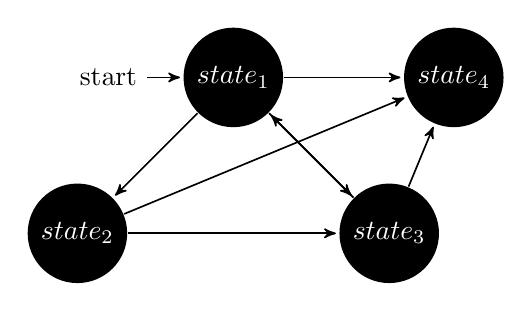
\begin{tikzpicture}[->,>=stealth',shorten >=1pt,auto,node distance=2.8cm,
                    semithick]
  \tikzstyle{every state}=[fill=black,draw=none,text=white]

  \node[initial,state] (state1)                    		{$state_1$};
  \node[state]         (state2) [below left of=state1] 	{$state_2$};
  \node[state]         (state3) [below right of=state1] {$state_3$};
  \node[state]         (state4) [right of=state1] 		{$state_4$};

  \path (state1) edge node {} (state2)
				 edge node {} (state3)
				 edge node {} (state4);
  \path (state2) edge node {} (state3)
				 edge node {} (state4);
  \path (state3) edge node {} (state1)
				 edge node {} (state4);			 
  
\end{tikzpicture}

\end{document}